\documentclass{standalone}
\usepackage{tikz}
\usetikzlibrary{positioning}
\begin{document}
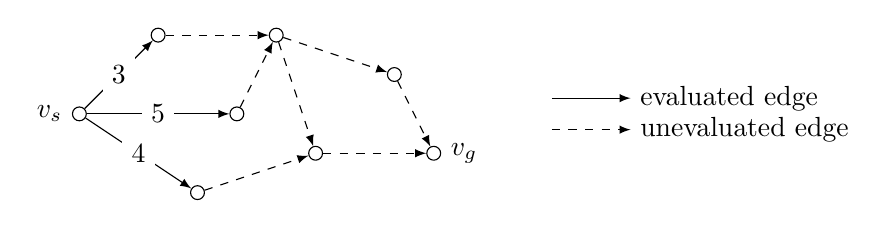
\begin{tikzpicture}
\tikzstyle{vertex}=[circle,draw=black,inner sep=0pt,minimum size=5pt]

\node[vertex] (a) at (0,0) {};
\node[vertex] (b) at (2,0) {};
\node[vertex] (c) at (2.5,1) {};
\node[vertex] (d) at (1,1) {};
\node[vertex] (e) at (3,-0.5) {};
\node[vertex] (f) at (4,0.5) {};
\node[vertex] (g) at (4.5,-0.5) {};
\node[vertex] (h) at (1.5,-1) {};

\draw[black,->,>=latex] (a) -- (b) node [midway, fill=white] {5};
\draw[black,->,>=latex] (a) -- (h) node [midway, fill=white] {4};
\draw[black,->,>=latex] (a) -- (d) node [midway, fill=white] {3};
\draw[black,->,dashed,>=latex] (b) -- (c);
\draw[black,->,dashed,>=latex] (d) -- (c);
\draw[black,->,dashed,>=latex] (c) -- (e);
\draw[black,->,dashed,>=latex] (c) -- (f);
\draw[black,->,dashed,>=latex] (f) -- (g);
\draw[black,->,dashed,>=latex] (e) -- (g);
\draw[black,->,dashed,>=latex] (h) -- (e);

\draw[black,->,>=latex] (6,0.2) -- (7,0.2);
\node[anchor=west] at (7,0.2) {evaluated edge};
\draw[black,->,dashed,>=latex] (6,-0.2) -- (7,-0.2);
\node[anchor=west] at (7,-0.2) {unevaluated edge};

\node[left=0pt of a] {$v_s$};
\node[right=0pt of g] {$v_g$};

\end{tikzpicture}%
\end{document}
